\documentclass[12pt]{article}

% --- Page geometry and spacing -------------------------------------------
\usepackage[letterpaper, margin=1in]{geometry}
\usepackage{setspace}
\onehalfspacing

% --- Typography ----------------------------------------------------------
\usepackage{times}
\usepackage[T1]{fontenc}
\usepackage[utf8]{inputenc}

% --- Math, graphics, tables ----------------------------------------------
\usepackage{amsmath, amssymb}
\usepackage{graphicx}
\usepackage{tikz}
\usepackage{tikz-3dplot}
\usepackage{pgfplots}
\usepackage{pgfplotstable}
\usepackage{tabularx}
\usepackage{booktabs}

% --- Section heading style (UW decimal numbering) ------------------------
\usepackage{titlesec}
\titleformat{\section}{\normalfont\Large\bfseries}{\thesection.0}{1em}{}
\titleformat{\subsection}{\normalfont\large\bfseries}{\thesubsection}{1em}{}
\titleformat{\subsubsection}{\normalfont\normalsize\bfseries}{\thesubsubsection}{1em}{}

% --- TOC, list of figures/tables -----------------------------------------
\usepackage{tocbibind}

% --- Hyperlinks (loaded last) --------------------------------------------
\usepackage[hidelinks]{hyperref}

% --- Page headers / footers ----------------------------------------------
\usepackage{fancyhdr}
\pagestyle{fancy}
\fancyhf{}
\fancyfoot[R]{\thepage}
\renewcommand{\headrulewidth}{0pt}

% =========================================================================
\begin{document}

% --- Title Page ----------------------------------------------------------
\begin{titlepage}
  \centering
  \vspace*{1.5cm}

  {\Large \textbf{Engineering Report:}\par}
  \vspace{0.4cm}
  {\Large \textbf{Design and Analysis of the 805 Electric Race Vehicle}\par}
  \vspace{0.4cm}
  {\large for the Waterloo EV Challenge\par}

  \vspace{2cm}
  
\includegraphics[width=0.4\textwidth]{EVC_logo.png}

  \vspace{2cm}
  \begin{tabular}{rl}
    \textbf{Prepared for:} & Laurel Heights Secondary School Electric Vehicle Club \\[0.3em]
    \textbf{Prepared by:}  & Ayden Chiu \\[0.3em]
                           & Bobby Liu \\[0.3em]
                           & Keaton McDermott \\[0.3em]
    \textbf{Race:}         & Waterloo EV Challenge \\[0.3em]
    \textbf{Submitted:}    & \today \\
  \end{tabular}

  \vfill
  {\small Laurel Heights Secondary School Electric Vehicle Club \\
   University of Waterloo}
\end{titlepage}

% --- Front matter (Roman numerals) ---------------------------------------
\pagenumbering{roman}
\setcounter{page}{2}

% --- Executive Summary ---------------------------------------------------
\section*{Executive Summary}
\addcontentsline{toc}{section}{Executive Summary}

Following the cancellation of the 24~V race category, the previous Laurel
Heights Secondary School (LHSS) Electric Vehicle Club race vehicle (803) is
no longer suitable for the 12~V race format. The October 2025 race
demonstrated that 803, equipped with a 48~V Saietta motor, could not sustain
race-duration battery life at 12~V supply. A new vehicle, designated 805, has
therefore been designed to address these limitations.

The 805 incorporates four major redesigns: a switch from steel to an aluminum
frame, reducing frame mass from 64.4~kg to 22.5~kg; an Ackermann steering
system in place of the previous anti-Ackermann geometry; two Kraken X60
brushless DC motors connected in parallel through a 9:1 gearbox and a 12:9
chain reduction (overall 12:1); and a new control system based on a
Raspberry Pi 4B running CTR Electronics' Phoenix6 framework with TalonFX
motor controllers over a CAN bus.

Quantitative analysis indicates that the 805 can operate continuously at
32.3~A on a single MTX-35 lead-acid battery for approximately 75~minutes,
based on Peukert's Law with a Peukert constant of 1.125 and a Peukert
capacity of 62.4~Ah. At cruise (43~km/h), the vehicle requires approximately
26.4~A combined motor current, leaving sufficient margin for transient loads
during turn re-acceleration and pit-stop restarts. Acceleration from 0 to
43~km/h is projected to require approximately 16.4~s with a 60~A-per-motor
burst current, while 27~to~43~km/h re-acceleration after each turn requires
approximately 6.4~s.

Combining the lap-time and energy-budget analyses, the 805 is projected to
complete approximately 40 laps of the 700~m course during the 70-minute
race, with a 5-minute energy reserve. Final performance figures will be
verified during physical testing prior to the October 2026 race.

\newpage

% --- Tables of Contents / Figures ----------------------------------------
\tableofcontents
\newpage
\listoffigures
\newpage

% --- Body (Arabic numerals) ----------------------------------------------
\pagenumbering{arabic}
\setcounter{page}{1}

% =========================================================================
\section{Introduction}

\subsection{Project Overview}
The performance of the previous LHSS EVC race vehicle, 803, in the Waterloo
EV Challenge October 2025 race was suboptimal. Although 803 led the race for
the first 15~minutes, the battery capacity deteriorated rapidly, resulting
in an inability to complete the race.

\subsection{Problem Statement}
The 803 vehicle was equipped with a single Saietta BR-119-R-68 motor, which
is designed for 48~V operation. According to the manufacturer's technical
specifications, this motor produces a torque of 12.1~Nm. However, due to the
characteristics of a 48~V-rated motor, it does not operate efficiently under
12~V usage. The motor consumed amperage in excess of expectations, which
contributed to 803's premature exit from the race. Additionally, the motor
weighs 11~kg, increasing the overall mass of the vehicle and therefore the
energy required for acceleration. Furthermore, 803 was equipped with an
anti-Ackermann steering system, which is not advantageous for the relatively
low-speed nature of this race.

\subsection{Design Objectives}
Following analysis of the previous race, the following design objectives
were established:
\begin{enumerate}
  \item Develop a new steering system that enables efficient turning;
  \item Increase the vehicle's top speed to above 35~km/h;
  \item Improve drivetrain efficiency such that the vehicle can complete the
        full race duration of 70~minutes;
  \item Reduce the overall mass of the vehicle.
\end{enumerate}

% =========================================================================
\section{Background}

\subsection{Competition Overview}
The competition is held in the parking lot adjacent to the East Campus of
the University of Waterloo. The race track measures approximately 700~m in
length and contains 3 major turns, as shown in Figure~\ref{fig:course}.

\begin{figure}[htbp]
  \centering
  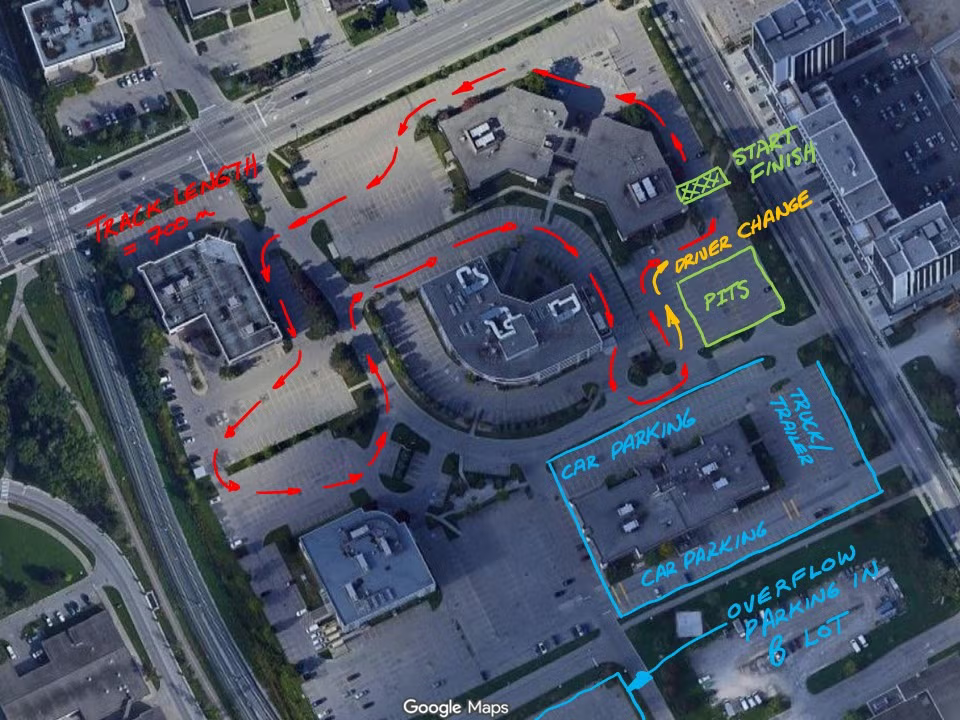
\includegraphics[width=0.7\textwidth]{Course.png}
  \caption{Race course layout for the May 2026 race.}
  \label{fig:course}
\end{figure}

\subsection{Design Constraints}
The rules governing the 2026 races are as follows:
\begin{enumerate}
  \item The distance between tires must be at least 0.90~m;
  \item Vehicle width must not exceed 1.2~m;
  \item Maximum vehicle length is 3.5~m;
  \item The driver must be in a seated, forward-facing position;
  \item The frame must possess sufficient structural strength to protect the
        driver;
  \item Two horizontal members spaced 6 to 10~inches apart must be installed
        to protect the driver's legs;
  \item Permitted frame materials are steel and aluminum;
  \item The roll bar must extend at least 50~mm above the top of the
        driver's helmet;
  \item The steering system must enable a turn within a radius of 5~m;
  \item Only the MTX-35 battery is permitted;
  \item The battery must be securely mounted;
  \item The driver must retain complete manual control of the vehicle.
\end{enumerate}

% =========================================================================
\section{Vehicle Design}

\subsection{Frame}

\subsubsection{Materials}

Previous vehicle generations used steel for their frames. However, this
material increased the overall mass of the vehicle. The current design
therefore adopts aluminum as the primary frame material.

According to simulation results, the frame mass is reduced from 64.4~kg to
22.5~kg. This significantly reduces the energy required to accelerate 805
to its top speed.

\subsubsection{Layout}

The 805 vehicle shares the same frame architecture as 804. The design
divides the vehicle into three sections: the leg, body, and back, as shown
in Figure~\ref{fig:car}.

\begin{figure}[htbp]
  \centering
  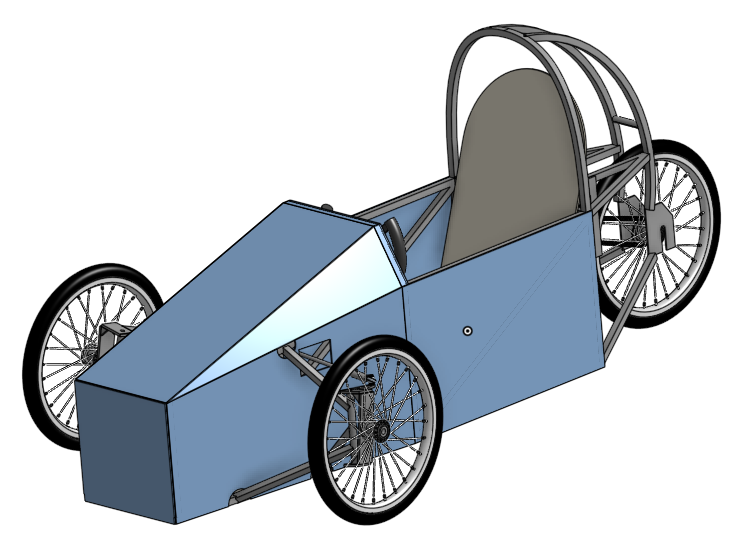
\includegraphics[width=0.7\textwidth]{Car.png}
  \caption{Overall design of the 805 vehicle.}
  \label{fig:car}
\end{figure}

\paragraph{Leg section.} The leg section is the front portion of the
vehicle. It accommodates the driver's legs, the steering system, and the
MTX-35 battery.

The battery is mounted at the front of the vehicle. This location provides
a more balanced weight distribution by counteracting the centre of mass of
the driver. The battery is held in place by a battery holder consisting of
two rods that secure the battery and four-sided barriers at the base, which
prevent the battery from displacing during operation
(Figure~\ref{fig:battery}).

\begin{figure}[htbp]
  \centering
  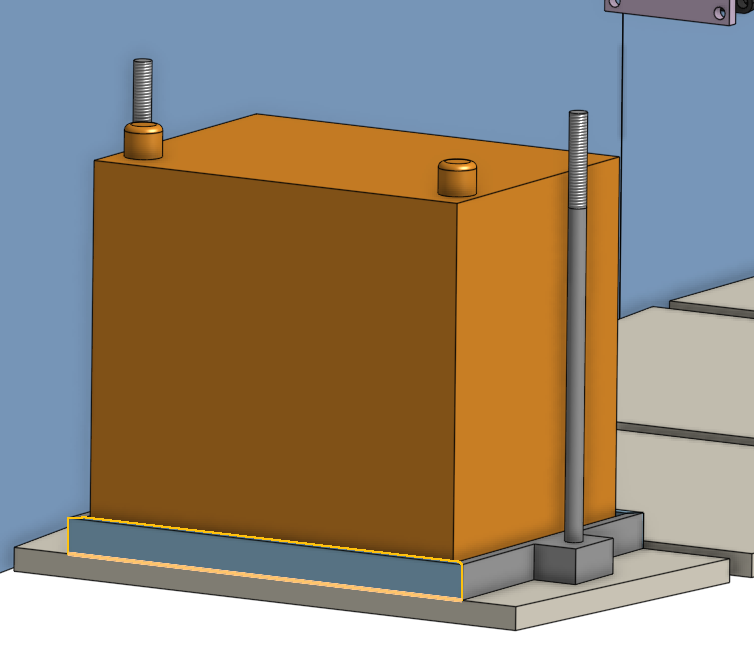
\includegraphics[width=0.3\textwidth]{Battery.png}
  \caption{Battery mounting design.}
  \label{fig:battery}
\end{figure}

A footrest is incorporated to prevent the driver from inadvertently
dislodging the battery from its mounted position
(Figure~\ref{fig:footrest}).

\begin{figure}[htbp]
  \centering
  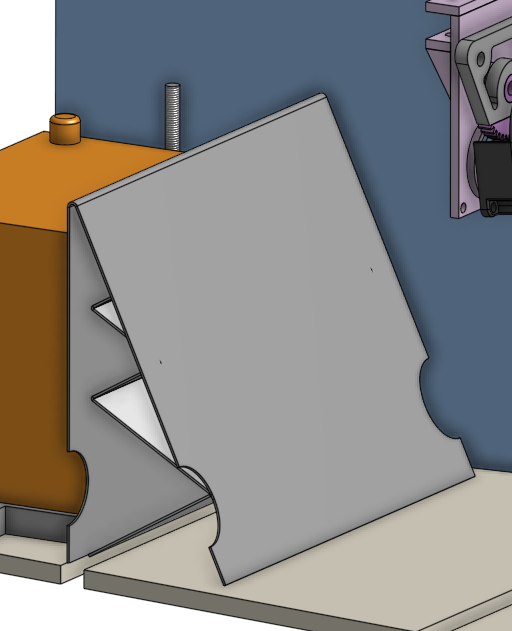
\includegraphics[width=0.3\textwidth]{footstep.png}
  \caption{Footrest design.}
  \label{fig:footrest}
\end{figure}

The steering gearbox is bolted to the middle-top crossbar
(Figure~\ref{fig:steeringloc}). Specific details regarding this gearbox are
discussed in Section~3.2.

\begin{figure}[htbp]
  \centering
  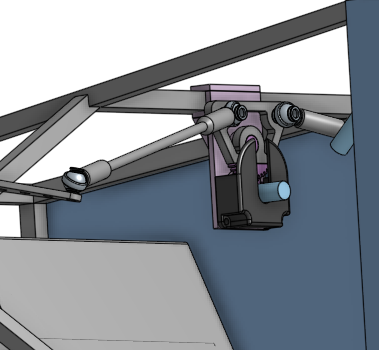
\includegraphics[width=0.4\textwidth]{steeringLoc.png}
  \caption{Steering gearbox location.}
  \label{fig:steeringloc}
\end{figure}

The leg section is enclosed by three panels (top, left, and right). These
panels are intended to streamline the vehicle and reduce the drag
coefficient (Figure~\ref{fig:leg}).

\begin{figure}[htbp]
  \centering
  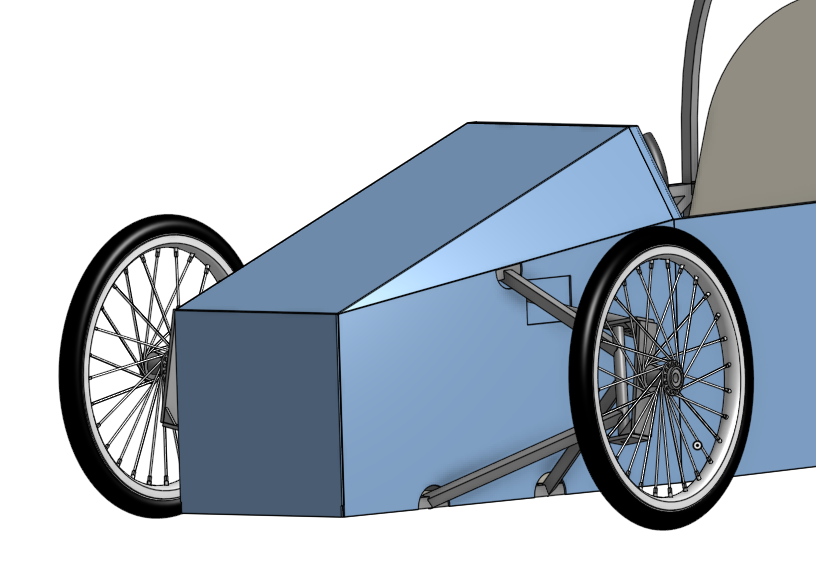
\includegraphics[width=0.4\textwidth]{leg.png}
  \caption{Front panel design.}
  \label{fig:leg}
\end{figure}

\paragraph{Body section.} The body section is where the driver sits and
operates the vehicle. This section contains the kill switch (highlighted in
yellow), the yoke, and the driver's seat (Figure~\ref{fig:body}).

The yoke is connected to three steering bars via two universal joints,
which together control the steering gearbox. The driver sits on a wood
plate inclined to both reduce the drag coefficient and enable the driver to
maintain a forward visibility of at least 2~m. The kill switch is located
on the right side of the driver to provide ready access in the event of an
emergency.

\begin{figure}[htbp]
  \centering
  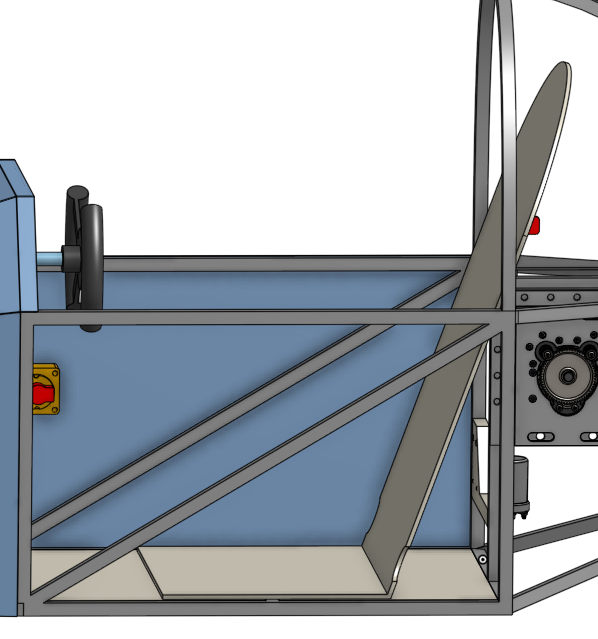
\includegraphics[width=0.4\textwidth]{body.png}
  \caption{Body section design.}
  \label{fig:body}
\end{figure}

\paragraph{Back section.} The back section of the vehicle houses all
components of the drivetrain. Two Kraken X60 motors are mounted to a
flipped gearbox, which is in turn attached to two mounting plates. After a
gear reduction of 9:1, the gearbox transfers rotational energy to a
sprocket connected to the rear wheel.

The two motors are connected via wiring to a CAN bus and a Raspberry Pi
control unit. These components are mounted on the panel located above the
rear wheel.

A roll cage extends from the bottom of the vehicle and arches over the
driver's helmet, providing a clearance of 50~mm for driver safety. Two bent
support beams connect the top of the roll cage to the rear mount of the
vehicle, as shown in Figure~\ref{fig:back}.

\begin{figure}[htbp]
  \centering
  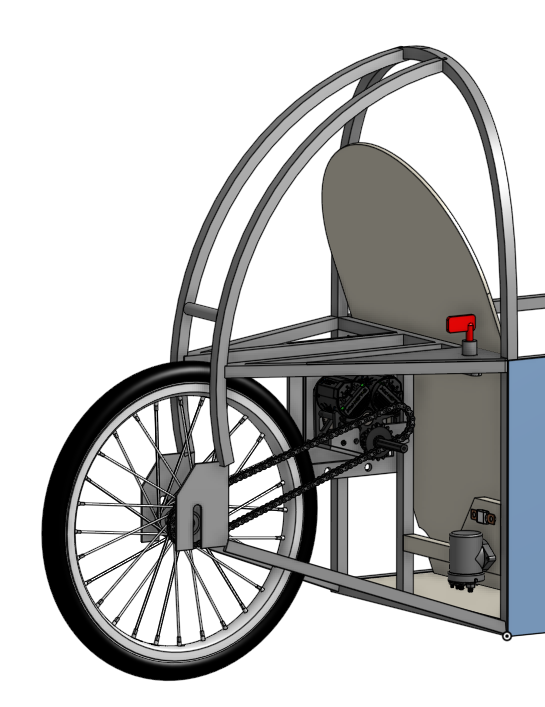
\includegraphics[width=0.4\textwidth]{back_section.png}
  \caption{Back section design.}
  \label{fig:back}
\end{figure}

The 805 is equipped with 19-inch diameter bicycle wheels at the two front
positions and the rear position. This selection facilitates effective
torque transfer from the motor to the ground. Furthermore, the bicycle
wheel design significantly reduces frictional losses, allowing the vehicle
to operate efficiently.

% -------------------------------------------------------------------------
\subsection{Steering System}

\begin{figure}[htbp]
  \centering
  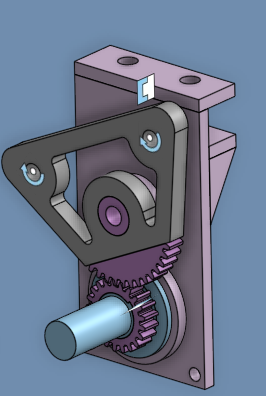
\includegraphics[width=0.3\textwidth]{steering_overview.png}
  \caption{Steering system overview.}
  \label{fig:steering}
\end{figure}

\textit{[Section to be completed: detailed description of the Ackermann
steering geometry, gearbox specifications, linkage dimensions, and turning
radius calculation.]}

% -------------------------------------------------------------------------
\subsection{Drivetrain}

\subsubsection{Overview}

In light of the unsatisfactory results of the October race, the team
concluded that 803 lacked the efficiency and energy required to complete
the race. Accordingly, a motor designed for 12~V operation was selected for
the 805 vehicle.

After preliminary research, the design team identified several industrial
motors rated for 12~V operation. However, none of the corresponding
manufacturers responded to inquiries, and this option was therefore not
pursued.

Robotics motors became the only viable option for the team. After
consultation with several FIRST robotics team members within the club, the
Kraken X60 was identified as the optimal motor for this application
\cite{ctrelectronics}. Other motors that were considered include the
Kraken X44, the NEO Vortex, and the NEO 2.0.

\subsubsection{Performance Data}

Using data acquired from publicly available sources, the performance graph
shown in Figure~\ref{fig:kraken} was generated to determine the operating
RPM, torque, and current of the Kraken X60.

\begin{figure}[htbp]
  \centering
  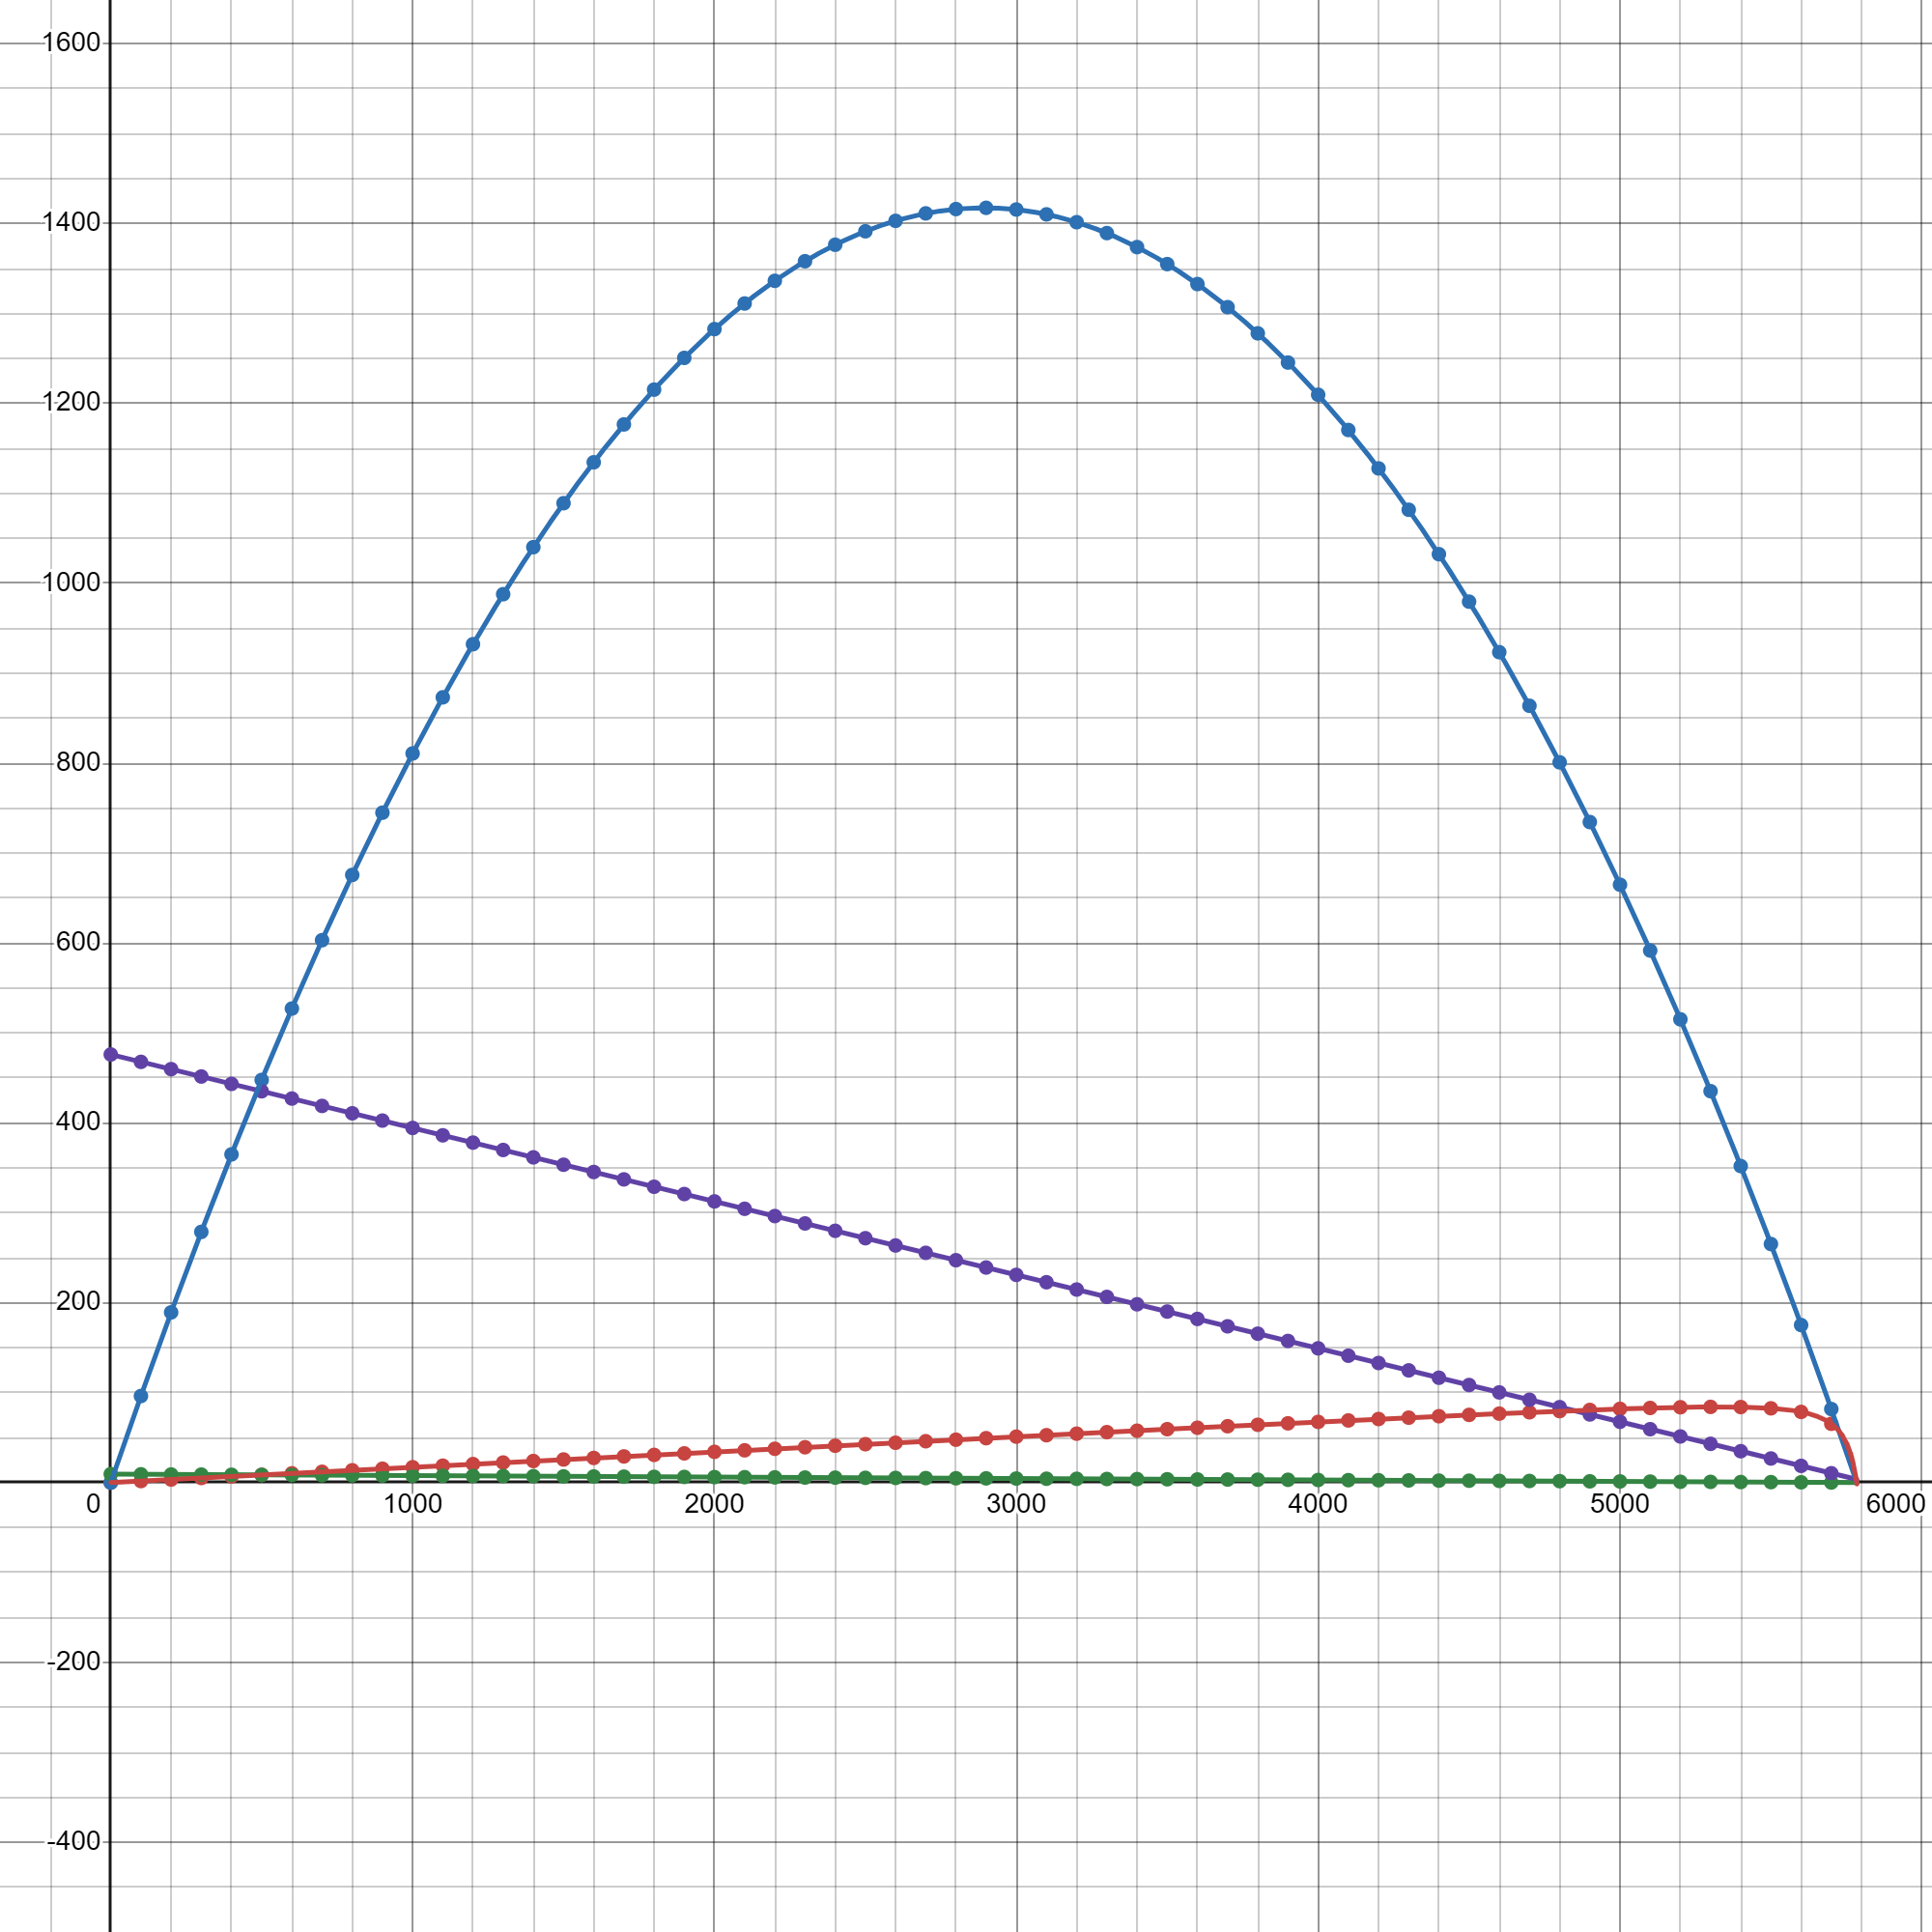
\includegraphics[width=0.6\textwidth]{Kraken X60.png}
  \caption{Kraken X60 performance characteristics.}
  \label{fig:kraken}
\end{figure}

The horizontal axis represents the motor RPM. The blue curve indicates the
output power (W); the purple curve indicates the current draw (A); the
green curve indicates the torque (Nm); and the red curve indicates the
efficiency. The interactive version of the graph is available at
\cite{krakengraph}.

% -------------------------------------------------------------------------
\subsection{Electrical Architecture}

\subsubsection{Phoenix6 Software Framework}

In order to control the two Kraken X60 motors, the Phoenix6 software
framework by CTR Electronics is used to interface with the TalonFX motor
controllers built into each motor \cite{phoenix6}. The RoboRIO, an
FRC-specific robotics controller, was not selected due to its cost. A
Raspberry Pi 4B was chosen instead to run the Phoenix6 framework.

The architecture of the entire drivetrain is shown in
Figure~\ref{fig:architecture}.

\begin{figure}[htbp]
  \centering
  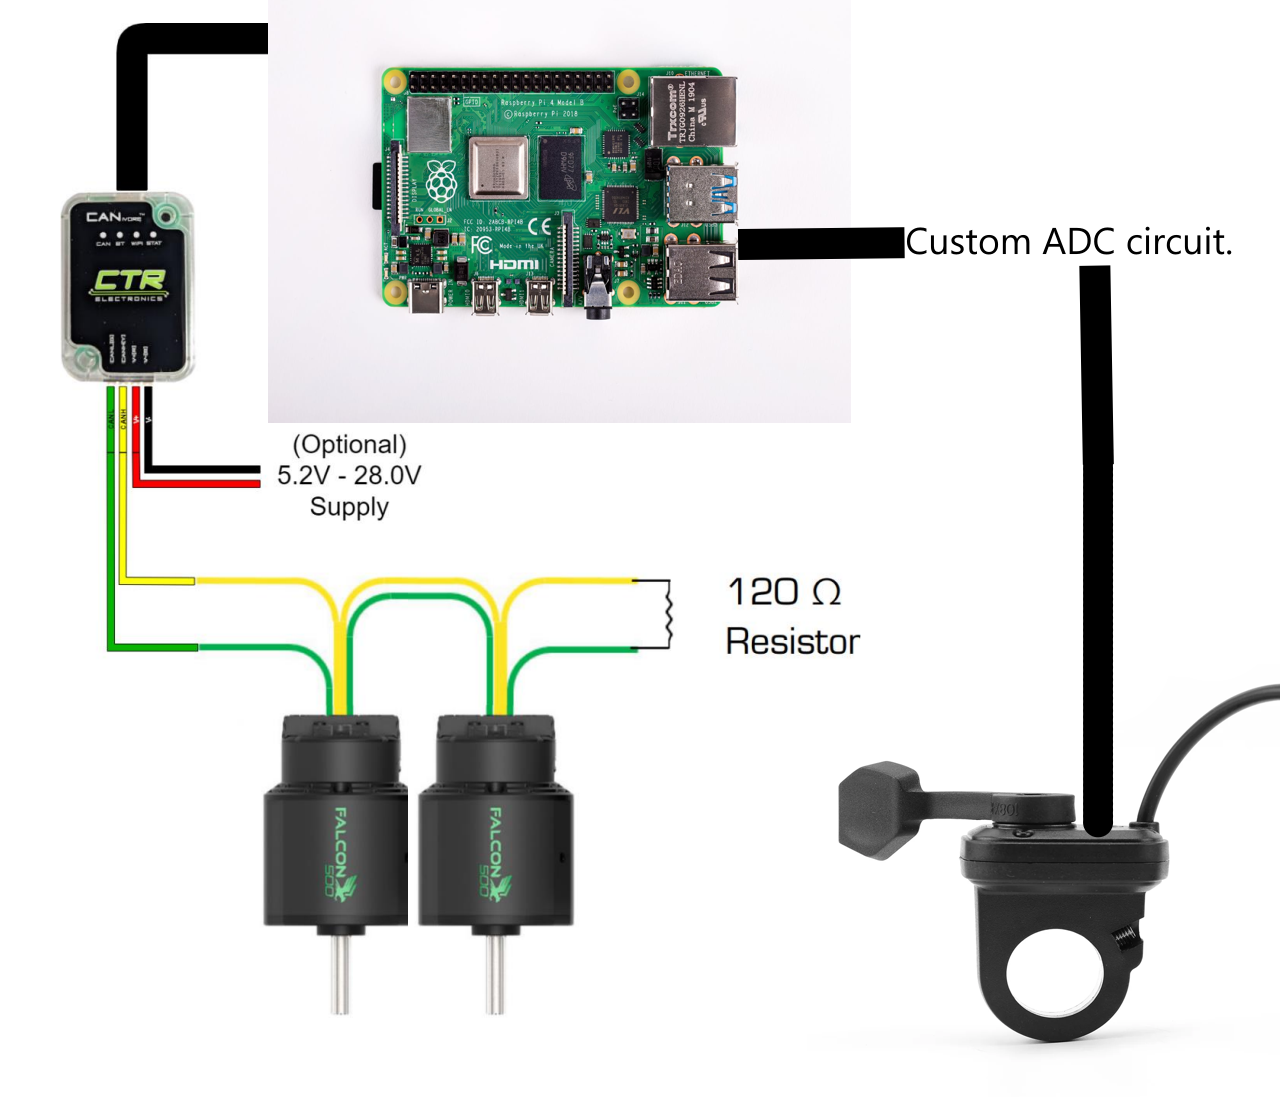
\includegraphics[width=0.5\textwidth]{DrivetrainArchitecture.png}
  \caption{Electric drivetrain architecture.}
  \label{fig:architecture}
\end{figure}

The system includes the following components:
\begin{enumerate}
  \item \textbf{Throttle:} input device that allows the driver to control
        the power delivered to the motors;
  \item \textbf{Analog-to-Digital converter:} a custom circuit that accepts
        a 0.8 to 4.2~V signal and outputs UART serial data to the
        Raspberry Pi;
  \item \textbf{Raspberry Pi 4B:} processes throttle data and transmits CAN
        frames over the CAN bus to control the motors;
  \item \textbf{Canivore:} a USB-to-CAN adapter manufactured by CTR
        Electronics;
  \item \textbf{Kraken X60:} two motors connected in tandem to drive the
        rear wheel of the vehicle.
\end{enumerate}

% =========================================================================
\section{Drivetrain Analysis}

\subsection{Maximum Continuous Current}

A preliminary calculation is required to determine the maximum continuous
current that can be delivered to the motors while ensuring that the vehicle
can complete the race.

The 12~V race format requires 805 to use a single MTX-35 battery. The
MTX-35 is an absorbent glass mat (AGM) lead-acid battery with the
specifications listed in Table~\ref{tab:mtx35} \cite{mtx35}.

\begin{table}[htbp]
  \centering
  \caption{MTX-35 battery specifications.}
  \label{tab:mtx35}
  \begin{tabular}{ll}
    \toprule
    \textbf{Parameter} & \textbf{Value} \\
    \midrule
    Mass                       & 18.1~kg \\
    Reserve capacity at 25~A   & 100~minutes (1.67~h) \\
    Nominal voltage            & 12~V \\
    Capacity (20-hour rate)    & 55~Ah \\
    Maximum current rating     & 800~A \\
    Chemistry                  & AGM lead-acid \\
    \bottomrule
  \end{tabular}
\end{table}

Lead-acid battery behaviour is more accurately represented by Peukert's Law
than by Watt's Law \cite{peukert}:
\begin{equation}
  C_p = I^k \times t
  \label{eq:peukert}
\end{equation}
where $C_p$ is the Peukert capacity (the equivalent capacity at a
one-ampere discharge rate, expressed in ampere-hours); $I$ is the actual
discharge current (in amperes) drawn by the load; $t$ is the actual
discharge time (in hours); and $k$ is the Peukert constant (dimensionless).

The Peukert constant $k$ is determined for the MTX-35 from
Equation~\ref{eq:k}:
\begin{equation}
  k = \frac{\log(t_2) - \log(t_1)}{\log(I_1) - \log(I_2)}
  \label{eq:k}
\end{equation}

Two discharge data points are obtained from the manufacturer's 20-hour rate
and reserve capacity rate. The 20-hour rate corresponds to the rated
capacity of 55~Ah, yielding a discharge current of 2.75~A. The reserve
capacity rate gives a discharge time of 1.67~h at 25~A. Substituting these
values into Equation~\ref{eq:k}:
\[
k = \frac{\log(1.67)-\log(20)}{\log(2.75)-\log(25)} = 1.125
\]

Using the calculated Peukert constant in Equation~\ref{eq:peukert}, the
maximum continuous current that can be drawn over the race is determined.
The race duration is taken to be 75~minutes (1.25~h), which provides a
5-minute reserve over the 70-minute target:
\[
2.75^{1.125} \times 20 = I_{race}^{1.125} \times 1.25
\]
\[
I_{race} = 32.3~\text{A}, \quad C_p = 62.4~\text{Ah}
\]

The 805 vehicle may therefore draw a maximum continuous current of 32.3~A,
with a Peukert capacity of 62.4~Ah.

\subsection{Motor Performance at Maximum Current}

Because the 805 employs two Kraken X60 motors connected in parallel through
a single flipped gearbox, the current per motor is approximately 16.2~A
continuous (half of the system current).

From the performance graph in Figure~\ref{fig:kraken}, each Kraken X60
operates at the following point at 16.2~A:
\begin{itemize}
  \item Power: 158.8~W;
  \item Efficiency: 76.7\%;
  \item RPM: 5624~RPM;
  \item Torque: 0.258~Nm.
\end{itemize}

For the parallel-connected pair, the combined performance is therefore
317.6~W of output power, 0.516~Nm of torque, and 5624~RPM at the motor
shaft.

The selected gearbox provides a 9:1 reduction (motor to gearbox output).
Its output is then coupled to the rear wheel through a chain drive with a
12:9 reduction (driving sprocket: 9 teeth on the gearbox output shaft;
driven sprocket: 12 teeth on the wheel). The overall reduction from motor
to wheel is therefore $9 \times \frac{12}{9} = 12{:}1$.

Applying the inverse relationship between torque and rotational speed
across a gear reduction:
\begin{equation}
  \frac{\tau_{input}}{\tau_{output}} = \frac{\text{Gear input}}{\text{Gear output}}
  \label{eq:torquegear}
\end{equation}
\[
\tau_{output} = 0.516 \times 12 = 6.192~\text{Nm}
\]
\begin{equation}
  \frac{RPM_{input}}{RPM_{output}} = \frac{\text{Gear output}}{\text{Gear input}}
  \label{eq:rpmgear}
\end{equation}
\[
RPM_{output} = \frac{5624}{12} = 468.7~\text{RPM}
\]

The wheel therefore operates at 468.7~RPM with an output torque of
6.192~Nm.

\subsection{Stages of the Race}

The race is run primarily at constant speed; however, turns and starts
affect the current drawn from the battery. Accordingly, the 805 must be
analyzed under the following three operating conditions:
\begin{enumerate}
  \item Cruise;
  \item Acceleration: 0--43~km/h (race start and after each pit stop);
  \item Acceleration: 27--43~km/h (recovery from each major turn).
\end{enumerate}

The current required to maintain a top speed of 43~km/h is determined using
Newton's second law applied to the vehicle:
\begin{equation}
  F_{net} = F_A - F_f - F_{AR}
  \label{eq:newton}
\end{equation}
where $F_{net} = ma$ is the net force on the vehicle; $F_A$ is the
propulsive force provided by the Kraken motors; $F_f$ is the rolling
resistance force opposing motion; and $F_{AR}$ is the aerodynamic drag
force opposing motion.

\subsubsection{Cruise}

At cruise, $F_{net} = 0$, hence:
\[
F_A = \mu mg + \tfrac{1}{2}\rho v^2 C_D A
\]

The parameters and assumptions used in this calculation are listed in
Table~\ref{tab:cruise}.

\begin{table}[htbp]
  \centering
  \caption{Cruise parameters and assumptions.}
  \label{tab:cruise}
  \begin{tabular}{lll}
    \toprule
    \textbf{Symbol} & \textbf{Description} & \textbf{Value} \\
    \midrule
    $\mu$  & Rolling resistance coefficient (bicycle on asphalt) & 0.005 \\
    $m$    & Total vehicle mass                                  & 116.5~kg \\
    $g$    & Gravitational acceleration                          & 9.81~m/s$^2$ \\
    $\rho$ & Air density                                          & 1.225~kg/m$^3$ \\
    $v$    & Velocity (43~km/h)                                  & 11.94~m/s \\
    $C_D$  & Drag coefficient                                     & 0.35 \\
    $A$    & Frontal cross-sectional area                         & 0.42~m$^2$ \\
    \bottomrule
  \end{tabular}
\end{table}

\[
F_A = (0.005)(116.5)(9.81) + \tfrac{1}{2}(1.225)(11.94)^2(0.35)(0.42)
    = 18.6~\text{N}
\]

The required propulsive force is therefore 18.6~N. Applying the
relationship between force at the wheel and torque:
\[
\tau = F_A \cdot r_{wheel} = 18.6 \times 0.2413 = 4.48~\text{Nm}
\]

After the 12:1 gear reduction and the parallel split between the two
motors, the torque required from each individual motor is approximately
0.187~Nm. The corresponding operating point read from the performance graph
(Figure~\ref{fig:kraken}) is summarized in Table~\ref{tab:cruisepoint}.

\begin{table}[htbp]
  \centering
  \caption{Cruise operating point per motor at 43~km/h.}
  \label{tab:cruisepoint}
  \begin{tabular}{ll}
    \toprule
    \textbf{Quantity} & \textbf{Value} \\
    \midrule
    Mechanical power per motor   & 111.0~W \\
    Efficiency                   & $\sim$70\% \\
    Current per motor            & 13.2~A \\
    Combined cruise current      & 26.4~A \\
    Motor RPM                    & 5680~RPM \\
    \bottomrule
  \end{tabular}
\end{table}

The combined cruise current of 26.4~A is well within the 32.3~A continuous
budget established in Section~4.1, leaving a margin for transient loads.

\subsubsection{Acceleration: 0--43 km/h}

This phase applies at the start of the race and after each pit stop, and
therefore occurs three times during the race. From a full stop, the 805
must accelerate to its cruise speed of 43~km/h. Applying
Equation~\ref{eq:newton} with $F_{net} = m(dv/dt)$:
\[
m \frac{dv}{dt} = F_A(I) - \mu mg - \tfrac{1}{2}\rho v^2 C_D A
\]

The continuous current limit of 16.2~A per motor is insufficient for
practical acceleration: at this current the propulsive force is only
25.7~N, giving an initial acceleration of 0.17~m/s$^2$ and a 0--43~km/h
time exceeding 90~seconds. The TalonFX motor controllers therefore permit
a short-duration current burst of approximately 60~A per motor (120~A
combined) during these acceleration phases, which is well within the
800~A maximum rating of the MTX-35.

At a burst current of 60~A per motor:
\begin{itemize}
  \item Torque per motor: $K_t \cdot I \approx 0.96$~Nm
        (using $K_t \approx 0.0159$~Nm/A);
  \item Combined wheel torque after 12:1 reduction: $\sim$23~Nm;
  \item Propulsive force at the wheel: $F_A \approx 95$~N;
  \item Initial acceleration: $a(0) \approx 0.77$~m/s$^2$.
\end{itemize}

Solving the resulting first-order ODE numerically yields a 0~to~43~km/h
time of approximately 16.4~s, a distance of approximately 100~m, and an
electrical energy consumption of approximately 6.5~Wh per start. Across
three pit-related starts, the total energy consumed during this phase is
approximately 19.5~Wh.

\subsubsection{Acceleration: 27--43 km/h}

This phase models the re-acceleration following each major turn. The
cornering speed is taken to be 27~km/h (7.50~m/s), which respects the
5~m turning radius constraint and provides safe lateral acceleration on
asphalt.

Using the same 60~A per motor burst current and the same governing
equation, the re-acceleration analysis yields a 27~to~43~km/h time of
approximately 6.4~s, a distance of approximately 63~m, and an electrical
energy consumption of approximately 2.5~Wh per turn exit.

The course contains 3 major turns per lap. The combined cruise and
turn-burst energy demand is the dominant factor in the lap-count estimate
presented in Section~5.

% =========================================================================
\section{Results}

The 805 is currently in late-stage development and will not be available to
participate in the May 2026 race. The vehicle is instead targeted for the
October 2026 race. Based on present calculations, the projected performance
characteristics are summarized in Table~\ref{tab:results}.

\begin{table}[htbp]
  \centering
  \caption{Projected performance characteristics of the 805.}
  \label{tab:results}
  \begin{tabular}{ll}
    \toprule
    \textbf{Parameter} & \textbf{Projected Value} \\
    \midrule
    Top speed (cruise)                  & 43~km/h \\
    Cornering speed                     & 27~km/h \\
    Acceleration time, 0--43~km/h       & $\sim$16.4~s \\
    Acceleration time, 27--43~km/h      & $\sim$6.4~s \\
    Maximum continuous current          & 32.3~A \\
    Cruise current (combined)           & 26.4~A \\
    Race duration target                & 70~min (with 5-min reserve) \\
    Number of pit stops                 & 3 (driver changes) \\
    Turning radius                      & \textit{[to be measured]} \\
    \bottomrule
  \end{tabular}
\end{table}

\subsection{Lap-Count Estimation}

The total number of laps is estimated by combining the lap-time analysis
with the energy budget over the 70-minute race.

\paragraph{Lap time.} The 700~m course is divided into a cruise segment of
approximately 271~m (where the vehicle holds 43~km/h) and three turn zones
of roughly 143~m each (deceleration, cornering at 27~km/h, and
re-acceleration). The estimated lap time is approximately 69~s.

\paragraph{Pit stops.} The race plan includes 3 pit stops for driver
changes. Each stop is estimated at approximately 30~s of stationary time,
plus a small additional time penalty due to 0--43~km/h re-acceleration
relative to cruise. The combined pit cost is approximately 90--115~s over
the race.

\paragraph{Time-limited lap count.} Subtracting pit time from the 4200~s
race duration and dividing by lap time yields an upper bound of
approximately 59~laps.

\paragraph{Energy-limited lap count.} Per-lap energy consumption is
approximately 10~Wh (dominated by the three turn re-accelerations), and
each pit-stop restart adds approximately 6.5~Wh. Against the 484.5~Wh
battery budget, this gives an upper bound of approximately 46~laps.

\paragraph{Conclusion.} Energy is therefore the binding constraint. After
applying a margin of approximately 10--15\% for real-world losses
(weather, manufacturing tolerances, voltage sag, and additional drag), the
805 is projected to complete approximately \textbf{40 laps} during the
70-minute race.

These figures are projections only. Actual values are subject to weather
conditions, additional friction, drag, voltage sag, and
manufacturing-related energy losses. Final results will be reported
following physical testing of the completed vehicle.

% =========================================================================
\section{Conclusions}

In order to remain competitive in the upcoming race, LHSS EVC has
redesigned the steering, electrical, and motor systems of the vehicle, as
well as the frame material, to maximize efficiency and motor power output.

The steering system has been changed from the anti-Ackermann configuration
used on 804 to an Ackermann configuration. This system is expected to
provide greater stability during turns and reduce tire slip, thereby
reducing drag in turns and allowing higher re-acceleration speeds following
each major turn.

The 805 incorporates two Kraken X60 motors, which operate natively at 12~V.
This configuration enables more efficient energy conversion. Because the
Kraken motors operate at high RPM, a reducing gearbox combined with a chain
drive (overall 12:1) is used to produce the torque and rotational speed
required at the wheel.

The new motor system also required a new wiring architecture. A CAN bus
control unit and a Raspberry Pi 4B running the Phoenix6 framework were
incorporated to program and command the motor controllers for optimal
efficiency.

The 805's frame material has been changed to aluminum, which has a lower
density and therefore lower mass than steel. This reduces the energy
required to accelerate and decelerate the vehicle, and the energy savings
contribute to higher acceleration and a higher top speed.

Quantitative analysis projects a top speed of 43~km/h, a 0--43~km/h
acceleration time of approximately 16~s under burst current, and
approximately 40 completed laps during the 70-minute race.

% =========================================================================
\section{Recommendations}

The following actions are recommended to validate and refine the 805
design:
\begin{enumerate}
  \item \textbf{Complete physical assembly} of the 805 vehicle in time for
        on-track testing prior to the October 2026 race.
  \item \textbf{Tune the burst current limits} in the TalonFX firmware
        (via Phoenix6) to balance acceleration time against energy
        consumption over the full race.
  \item \textbf{Implement telemetry logging} (motor current, voltage, RPM,
        battery state of charge) so that race data can be used to refine
        the model for the next vehicle generation.
\end{enumerate}

% =========================================================================
\newpage

\begin{thebibliography}{9}

\bibitem{ctrelectronics}
CTR Electronics, ``Kraken X60 brushless motor product page,'' 2025.
[Online]. Available: \url{https://store.ctr-electronics.com/kraken-x60/}.

\bibitem{krakengraph}
A. Chiu, ``Kraken X60 performance characteristics (Desmos),'' 2026.
[Online]. Available: \url{https://www.desmos.com/calculator/baupqlsyxa}.

\bibitem{phoenix6}
CTR Electronics, ``Phoenix 6 software framework documentation,'' 2025.
[Online]. Available: \url{https://pro.docs.ctr-electronics.com/}.

\bibitem{mtx35}
Motomaster, ``MTX-35 AGM battery specification sheet,'' Canadian Tire, 2025.

\bibitem{peukert}
W. Peukert, ``\"Uber die Abh\"angigkeit der Kapazit\"at von der
Entladestromst\"arke bei Bleiakkumulatoren,'' \emph{Elektrotechnische
Zeitschrift}, vol.~20, pp.~287--288, 1897.

\end{thebibliography}

\end{document}
